\chapter{Conclusiones y trabajos futuros}
\label{cap_conclusiones}
El propósito de este capítulo es exponer las experiencias obtenidas a la largo del trabajo y la visión futura que tenemos de este.

\section{Conclusiones}
	Las experiencias obtenidas del trabajo son generalmente buenas, el autor considera haber cumplido todos los objetivos inicialmente propuestos
	y en muchos casos haberlos sobrepasado. 
	\par
	Durante el desarrollo del software de adquisición  se han adquirido y reforzado multitud de conocimientos. Las experiencias obtenidas del
	trabajo conjunto con el equipo de CALMA han sido muy positivas. El diseño del software ha sido muy condicionado por el hardware ya existente,
	en sistemas empotrados estos dos están muy enlazados. El autor no considera esto como una desventaja sino como una ventaja. Raras veces en
	proyectos reales uno tiene libertad total, la mayoría de veces uno se ve forzado  a colaborar y adaptarse a las limitaciones que le son
	impuestas. Además el colaborar con personas conlleva el aprender muchas cosas nuevas. Veamos el impacto que han tenido algunas de las
	decisiones que hemos tomado.
	\par
	La BeagleBone Black ha sido una de las cosas que nos han sido impuestas, sin embargo hemos tenido la libertad de elegir la distribución Linux.
	Entre Angstrom y Debian, las dos distribuciones oficiales que la placa soporta, nos quedamos con la primera. A pesar de haber cumplido todas
	nuestras necesidades esta no es una distribución muy popular y pocas personas están acostumbradas a trabajar con ella. Encontrar información o
	ayuda también ha sido desafiante debido a la pequeña comunidad de usuarios. Con respeto a esta elección podemos decir que no estamos
	arrepentidos, sin embargo no es la mejor elección que pudimos tomar. 
	\par
	El desarrollo del software de adquisición en Python es una elección que el autor considera afortunada. El gran numero de librerías, la gran
	comunidad existente y todas las propiedades inherentes del lenguaje han permitido avanzar rápidamente en el proceso de implementación. El
	código generado es claro, corto e intuitivo. La librería de \emph{AdaFruit}\cite{AdaFruitGit} nos ha permitido operar sobre las cabeceras de
	extensión de la BeagleBone Black de forma fácil e intuitiva.    
	\par
	Otra elección que consideramos afortunada es utilizar Sqlite\cite{Sqlite} para la base de datos local. Este sistema de gestión de bases de
	datos relacionales es muy ligero cosa que lo hace muy adecuado para nuestro trabajo.
	\par
	La realización de la herramienta Web también ha sido una experiencia agradable en la que hemos adquirido multitud de conocimientos nuevos. A
	diferencia del software de adquisición en la realización de esta hemos tenido más libertad a la hora del diseño. Veamos el impacto que han
	tenido algunas de las decisiones que hemos tomado. Obviaremos alguna elecciones como la arquitectura \emph{Modelo Vista Controlador} porque
	son muy triviales y existe gran cantidad de literatura disponible.
	\par
	Utilizar Zendframework y Apigility para la realización del \emph{back-end} ha sido una elección buena, sin embargo el autor no esta
	completamente satisfecho. La combinación entre framework y herramienta han facilitado y acelerado el proceso de implementación. Sin embargo
	los primeros pasos han sido un poco confusos, el autor considera que este es un framework muy completo pero también muy complicado para
	principiantes.
	\par
	La realización del \emph{front-end} en Sencha ExtJs es una elección que el autor considera afortunada. El framework es muy completo y en
	muchos casos implementa todo lo que una aplicación Web pueda necesitar. Trabajar con este ha sido muy fácil e intuitivo, incluso para un
	principiante. El único inconveniente ha sido el módulo de gráficos, el framework ofrece un módulo que nos permite crear gráficos. La
	funcionalidad es la misma que la ofrecida por HighStock, es fácil de usar, los gráficos son bellos estéticamente e interactivos. Sin embargo
	el modulo no se comporta bien ante la necesidad de representar un gran número de datos. Para sobrevenir este problema recurrimos a HighStock.
	\par
	HighStock es una elección con la que estamos muy satisfechos. La funcionalidad ofrecida ha cubierto todos nuestros requisitos. Además trabajar
	con el framework ha sido un placer, este es muy intuitivo y podemos encontrar múltiples ejemplos de uso.
	\par
	A continuación procederemos a detallar los resultados conseguidos en este trabajo. Empezaremos por el software de adquisición. Conjuntamente
	al sistema de adquisición actual e intentando interferir lo menos posible hemos desplegado el nuevo sistema de adquisición. El objetivo es
	identificar y eliminar posibles malfuncionamientos que puedan presentarse. El nuevo sistema de adquisición lleva operando de forma parcial
	desde el 25 de febrero de 2015. Acabamos de utilizar la palabra parcial porque hay algunas funcionalidades que no explotamos. La primera de
	estas es el barómetro. Un barómetro como el BM35 es muy caro, además el proceso de calibración y certificación puede ser aún más costoso. Al
	no tener barómetro no podemos generar los datos corregidos por presión. Actualmente estamos trabajando en alguna solución que permita a dos o
	más sistemas de adquisición compartir un barómetro. La segunda funcionalidad que no explotamos son los anchos de pulso. Como explicamos en el
	capítulo de introducción el nuevo sistema esta diseñado para hacer uso de un circuito de adaptación que genera pulsos cuyo ancho es
	proporcional a la energía de la señal. Estos circuitos no están listos, en su lugar seguimos utilizando los viejos que generan pulsos cuyo
	ancho es fijo. Debido a esto los histogramas de ancho de pulso carecen de significado. 
	\begin{figure}[h]
		\centering
		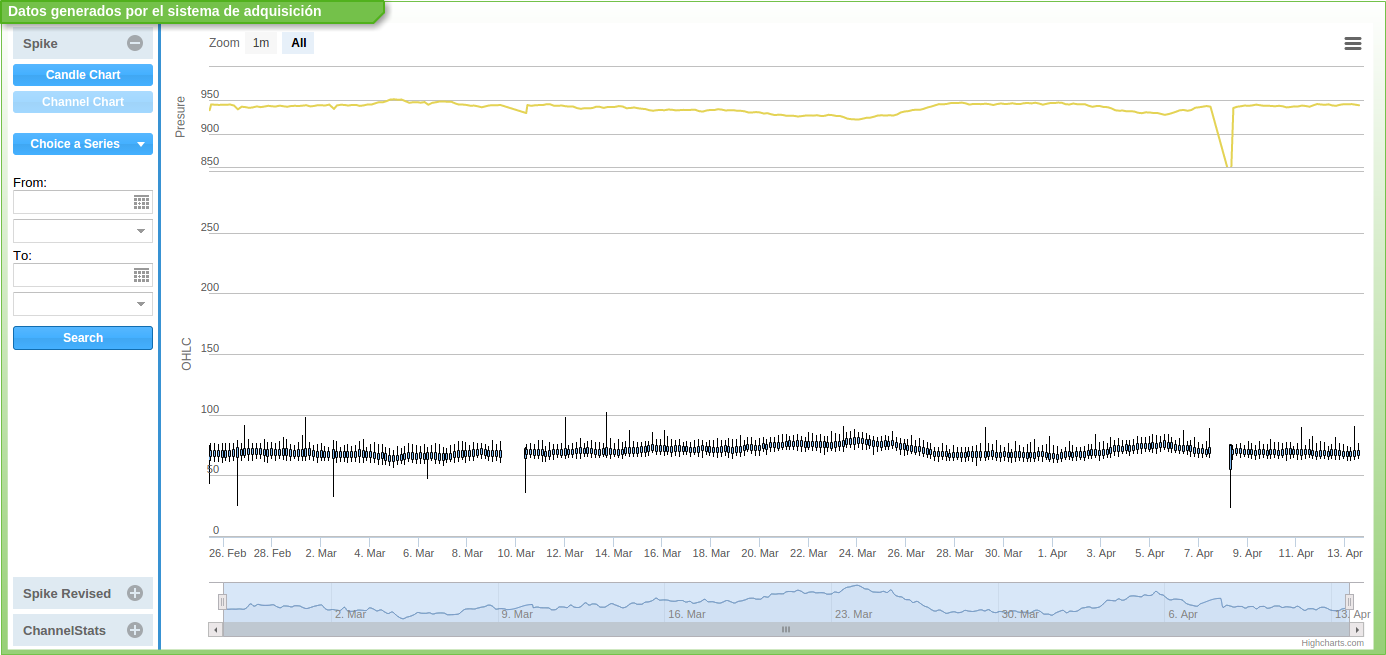
\includegraphics[keepaspectratio, width=1\textwidth]{./img/resultados.png}
		\caption{Datos generados por el sistema de adquisición.}   
		\label{fig:resultados}
	\end{figure}
	\par
	En la figura \ref{fig:resultados} podemos ver una captura de la herramienta Web, el gráfico es generado con los datos producidos por el
	sistema de adquisición. En relación a la herramienta Web podemos decir poco debido a que no hemos realizado un uso real de esta, recordamos
	que en este trabajo tan solo nos centramos en el proceso de desarrollo. Sin embargo basándose en las opiniones recibidas podemos decir que la
	herramienta tiene un futuro prometedor.

\section{Trabajos futuros}
	A pesar de estar satisfecho con los resultados conseguidos en este proyecto, este podría desarrollarse más.
	\par
	Tanto el software de adquisición como la herramienta Web han sido desarrollados en el entrono de CALMA, siendo condicionados por las
	características propias de la estación. Un ejemplo es el barómetro BM35 utilizado en CALMA, en otras estaciones son utilizados otros
	barómetros. Proponemos como trabajo futuro extender y adaptar tanto el sistema de adquisición como la herramienta Web para otras estaciones.
	Volvemos a hacer hincapié, al ser este un sistema empotrado el hardware también podría sufrir modificaciones. Este proceso implicaría
	implantar y mantener el sistema de adquisición en estas estaciones.
	\subsection{Software de adquisición}
		A continuación son detalladas una serie de mejoras y cambios que el software de adquisición podría experimentar a fin de mejorar.
		\begin{description}[style=unboxed,leftmargin=0cm,labelwidth=1cm]
			\item[Debian]
				Para la realización del software de adquisición hemos utilizado Angstrom, la distribución que viene por defecto con la
				BeagleBone Black. Esta es una distribución muy ligera y adecuada, pero la comunidad de usuarios es muy pequeña.
				Proponemos como trabajo futuro cambiar la Angstrom a alguna distribución derivada de Debian. Actualmente existen
				distribuciones basadas en Debian que son compatibles con las placas, gran parte de los usuarios instalan estas
				distribuciones en sus placas. El fabricante también ha anunciado que en un futuro las placas serán distribuidas con un
				Debian por defecto. El inconveniente que este cambio presenta, razón por la que no ha sido realizado en este trabajo,
				es que el software existente tendría que sufrir algunos cambios a fin de adaptarse al nuevo entorno.
				\par
				Actualmente el núcleo Linux y todo el sistema de archivos son cargados desde la memoria interna de la placa a la que
				nos referimos con el acrónimo eMMC. Es posible albergar la nueva distribución en la tarjeta microSD. El contenido de
				la tarjeta uSD es fácilmente duplicable, podemos exportar este a un archivo de imagen que contendría una copia exacta.
				Seguidamente podemos grabar este archivo de imagen en una nueva uSD. De esta manera todo el proceso descrito en el
				apéndice \ref{app_soft} queda obsoleto, para desplegar el software de adquisición  tan solo tenemos que grabar un
				archivo de imagen un una tarjeta uSD e introducirla en la ranura de la BeagleBone Black. 
		\end{description}
	\subsection{Herramienta Web}
		A continuación son detalladas una serie de mejoras y cambios que la herramienta Web podría experimentar a fin de mejorar.
		\begin{description}[style=unboxed,leftmargin=0cm,labelwidth=1cm]
			\item[Extender el soporte de navegación por el historial]
				En el capitulo dedicado al \emph{front-end} comentamos que el soporte de navegación por el historial es algo pobre.
				Proponemos como trabajo futuro extender esta funcionalidad. Actualmente tan solo son registrados los cambios entre
				módulos funcionales, es deseable que sean registrados más cambios como los intervalos temporales presentados en los
				gráficos. De esta manera utilizando los botones de navegación podríamos volver al estado anterior del gráfico.
			\item[Anchos de pulso] 
				Tal y como explicamos anteriormente en este trabajo el nuevo sistema de adquisición registra los anchos de los pulsos,
				anchos que son proporcionales a la energía de la señal original. Con estos datos son construidos histogramas con una
				resolución de 10 minutos. Estos histogramas son guardados en la base de datos en forma de cadenas Json. Proponemos
				como trabajo futuro extender la herramienta con un módulo funcional que permita visualizar estos datos. Para este
				propósito debemos encontrar la manera más efectiva de presentar los datos.  Al igual que el resto de la herramienta
				este módulo debe ser intuitivo e altamente interactivo. El módulo debe permitirnos especificar diferentes intervalos
				temporales, ocultar/mostrar series y mucho más.
			\item[Configuración del sistema de adquisición]
				Proponemos como trabajo futuro extender la herramienta con un módulo funcional que permita cambiar la configuración
				del sistema de adquisición en tiempo real. Recordemos del capítulo \ref{cap2} el archivo de configuración en el que
				definimos una serie de variables que configuran el software de adquisición. El módulo funcional que proponemos debería
				permitirnos cambiar el valor de estas variables sin interrumpir el proceso de adquisición. El desarrollo de este
				módulo tendrá que ser acompañado por el avance del software de adquisición. Este debe ofrecer una interfaz que permita
				esta configuración remota.
			\item[Alarmas y Notificación]
				Proponemos como trabajo futuro realizar un módulo funcional que genere alarmas y notificaciones. El módulo funcional
				debe ser capaz de detectar malfuncionamientos y tomar las acciones oportunas para informar al equipo de la estación.
				No generar datos o generar datos anormales son algunos ejemplos de malfuncionamiento.
			\item[Autenticación y autorización]
				Actualmente la herramienta Web no ofrece ningún servicio de acción, salvo el que nos permite eliminar Spikes. Podemos
				ver que planeamos realizar más de estos servicios de acción y esto puede ser un problema. Si queremos hacer que la
				herramienta sea accesible desde Internet debemos implementar algún mecanismo de autenticación y autorización. Los
				servicios de consulta serian accesible por todos los usuarios, sin embargo los servicios de acción serian accesible
				tan solo para los usuarios autorizados.
			\item[Implantación y Mantenimiento]
				En el capitulo de introducción especificamos los objetivos de este trabajo, entre estos objetivos tan solo
				contemplamos el desarrollo de la herramienta. Proponemos como trabajo futuro el implantar y mantener el software que
				compone la herramienta Web. 

			
		\end{description}
